% !TeX root = ./PA.tex
\documentclass[headheight=21.75pt,footheight=21.75pt]{scrartcl}

\usepackage{graphicx,tabularx,xcolor,hyperref,scrlayer-scrpage,scrhack,enumitem,listings,xurl,pdfpages,courier,anyfontsize,csquotes,fontspec}
\usepackage[style=apa]{biblatex}
\usepackage[top=30mm,bottom=30mm,left=40mm,right=35mm]{geometry}
\usepackage[printonlyused]{acronym}
\usepackage[nonumberlist]{glossaries}
\usepackage[english,ngerman]{babel}

\DeclareLanguageMapping{ngerman}{ngerman-apa}
\bibliography{PA}
\linespread{1.5}
\clubpenalty10000
\widowpenalty10000
\setcounter{biburllcpenalty}{7000}
\setcounter{biburlucpenalty}{8000}
\makeatletter
\lst@AddToHook{TextStyle}{\let\lst@basicstyle\ttfamily\normalsize}
\lst@AddToHook{DisplayStyle}{\let\lst@basicstyle\ttfamily\fontsize{8pt}{9.6pt}\selectfont}
\makeatother
\makeatletter
\renewcommand{\@pnumwidth}{3em}
\renewcommand{\@tocrmarg}{4em}
\makeatother
\lstset{breaklines=true,backgroundcolor=\color[HTML]{FFFFC0},literate={\_}{}{0\discretionary{\_}{}{\_}}}
\urlstyle{tt}
\DefineBibliographyStrings{ngerman}{nodate = {{}o. J.}}
\setlist{nosep,style=sameline}
\renewcommand{\sectionmark}[1]{\markboth{#1}{}}
\ihead{\leftmark}
\chead{}
\ohead{\autor}
\ifoot{}
\cfoot{\thepage}
\ofoot{}

\input hilfe/Einstellungen
\input inhalt/Glossar

\begin{document}

\fontsize{12.5pt}{15pt}\selectfont
\pagenumbering{Roman}
\input hilfe/Deckblatt
%\newpage \input hilfe/Sperrvermerk
\newpage \input hilfe/Erklaerung
\newpage \input inhalt/Abstract
\newpage \tableofcontents
\input inhalt/Abkuerzungen
\newpage \addcontentsline{toc}{section}{Abbildungsverzeichnis} \listoffigures
\newpage \addcontentsline{toc}{section}{Listings} \lstlistoflistings{}
\newpage \pagenumbering{arabic}
\input inhalt/1
\newpage \addcontentsline{toc}{section}{Literatur} \printbibliography{}
\newpage \addcontentsline{toc}{section}{Glossar} \glsaddall{} \printglossaries{}
\newpage \section*{Anmeldung} \addcontentsline{toc}{section}{Anmeldung} 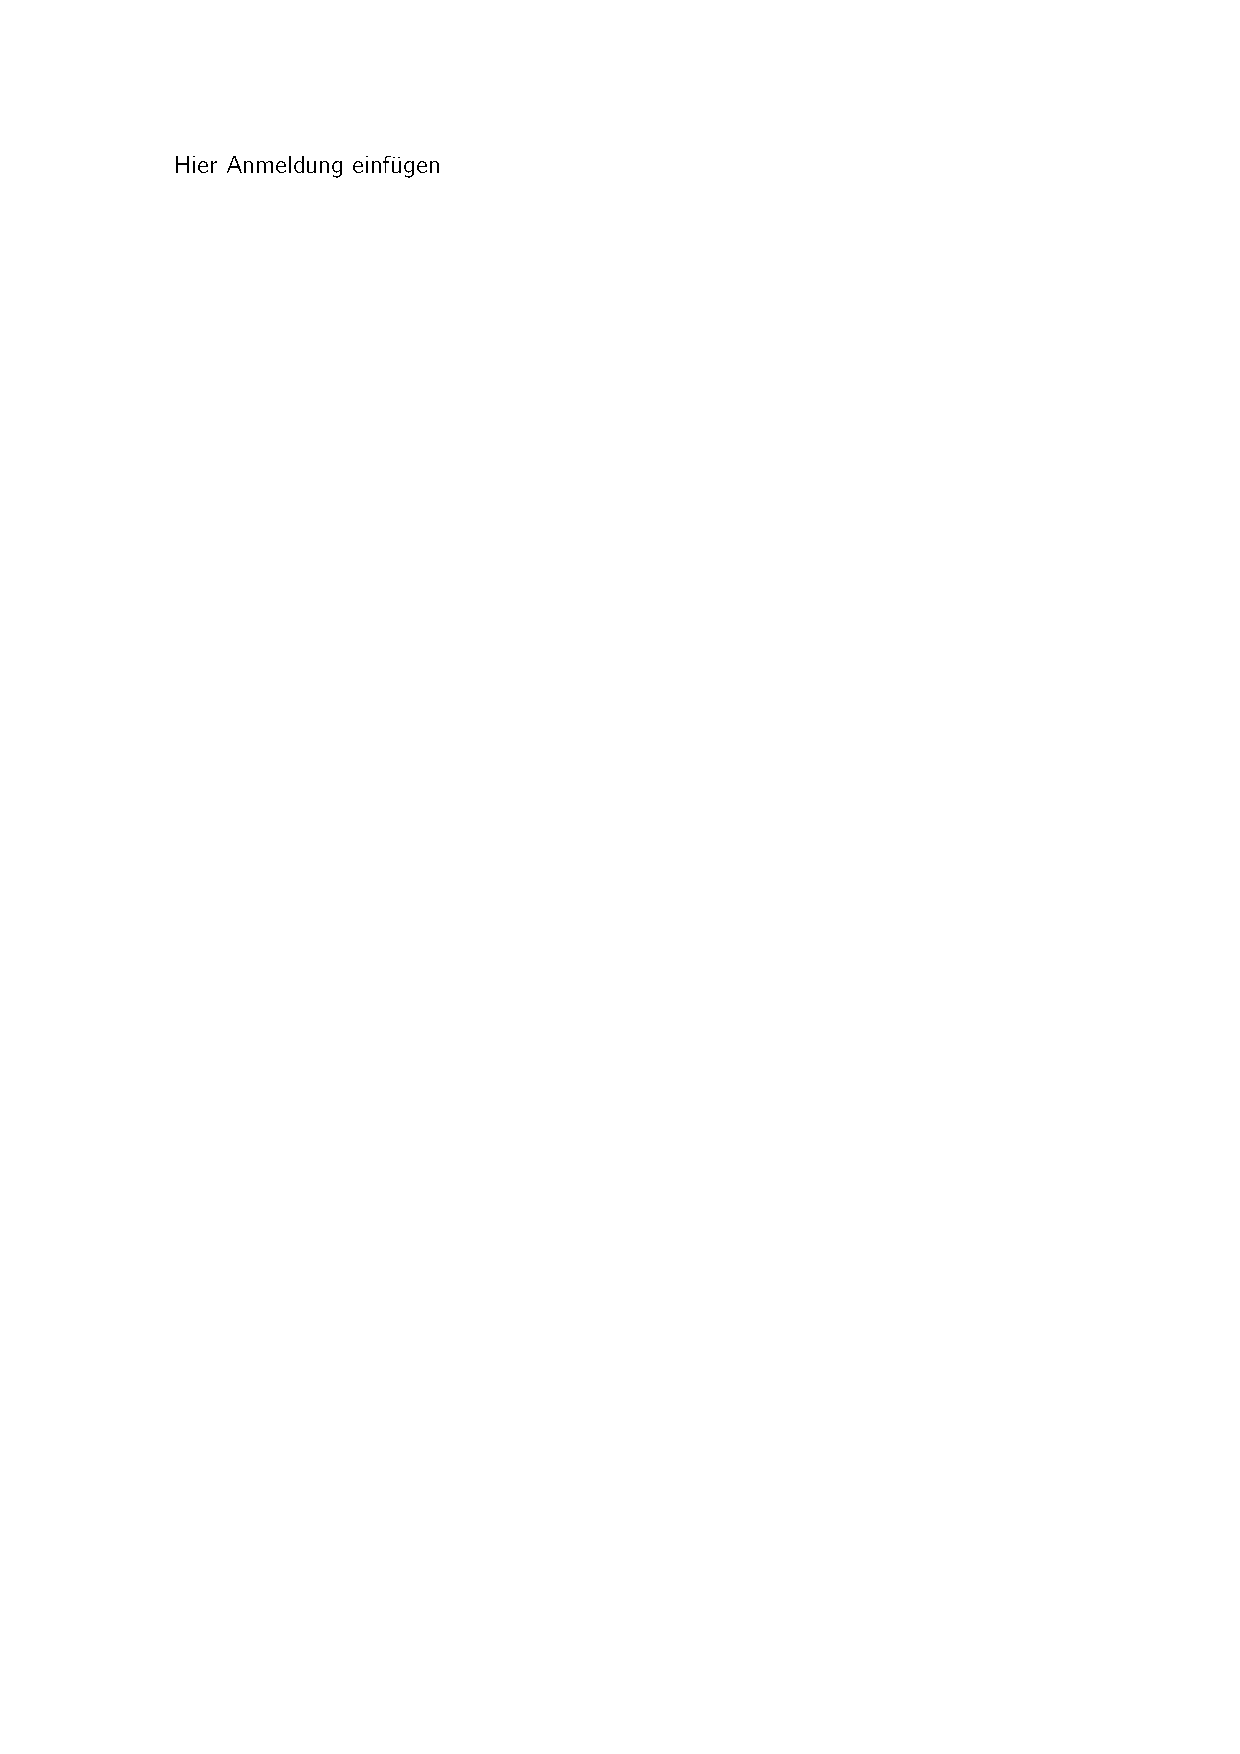
\includegraphics[width=\textwidth,trim= 60 60 60 60]{pdfs/anmeldung.pdf}

\end{document}
